\documentclass{article}
\setlength{\parskip}{0pt} % esp. entre parrafos
\setlength{\parindent}{20pt} % esp. al inicio de un parrafo
\usepackage{amsmath} % mates
\usepackage{listings}
\usepackage{xcolor}
\usepackage[sort&compress,numbers]{natbib} % referencias
\usepackage{url} % que las URLs se vean lindos
\usepackage[top=10mm,left=20mm,right=20mm,bottom=25mm]{geometry} % \textbf{\textbf{}}margenes
\usepackage{hyperref} % ligas de URLs
\usepackage{graphicx} % poner figuras
\usepackage{caption}
\usepackage{subcaption}
\usepackage[spanish]{babel} % otros idiomas
\hypersetup{
    colorlinks=true,
    linkcolor=blue,
    filecolor=blue,      
    urlcolor=blue,
}
\renewcommand{\lstlistingname}{C\'odigo}
\definecolor{codegreen}{rgb}{0,0.6,0}
\definecolor{codegray}{rgb}{0.5,0.5,0.5}
\definecolor{codepurple}{rgb}{0.58,0,0.82}
\definecolor{backcolour}{rgb}{0.95,0.95,0.92}
\lstdefinestyle{mystyle}{
    backgroundcolor=\color{backcolour},   
    commentstyle=\color{codegreen},
    keywordstyle=\color{magenta},
    numberstyle=\tiny\color{codegray},
    stringstyle=\color{codepurple},
    basicstyle=\ttfamily\footnotesize,
    breakatwhitespace=false,         
    breaklines=true,                 
    keepspaces=true,                 
    numbers=left,                    
    numbersep=5pt,                  
    showspaces=false,                
    showstringspaces=false,
    showtabs=false,                  
    tabsize=2
}
\lstset{style=mystyle}

\title{Reporte 3:\\Teor\'ia de Colas}
\author{Jorge Torres}
\date{\today}

\begin{document}

\maketitle

\section{Objetivo}\label{obj}
El objetivo de la pr\'actica consiste en analizar los tiempos de ejecuci\'on de tres algoritmos diferentes que encuentran si un n\'umero es primo. Se var\'ian tanto el algoritmo utilizado como el orden inicial de la lista de n\'umeros de forma independiente y se realiza un an\'alisis estad\'istico relevante para decidir si la diferencia en tiempos de ejecuci\'on es significativa o no. Por \'ultimo, se muestran resultados de la evaluaci\'on en gr\'aficas tipo viol\'in para una mejor interpretaci\'on.

\section{Desarrollo}\label{des}
Basando el desarrollo en el \href{https://github.com/satuelisa/Simulation/blob/master/QueuingTheory/ordering.py}{c\'odigo} implementado por E. Schaeffer \cite{elisa1}, primero se definen los par\'ametros de ejecuci\'on de los algoritmos, como se observa en el c\'odigo \ref{codigo1},

\begin{lstlisting}[caption=Par\'ametros, label=codigo1, language=Python]
d = 1000
h = 5000
replicas = 30
original = [x for x in range(d, h + 1)]
invertido = original[::-1]
aleatorio = original.copy()
shuffle(aleatorio)
\end{lstlisting}
donde se crea una lista de n\'umeros desde 1000 hasta 5000, y se establece que los experimentos tendr\'an 30 r\'eplicas. Los par\'ametros \texttt{invertido} y \texttt{aleatorio} simplemente reordenan la lista de n\'umeros de forma invertida y aleatoria, respectivamente.\\

Lo siguiente es definir las tres formas en que se decide si los n\'umeros son primos o no. Para esto se toman los \href{https://satuelisa.github.io/simulation/p3.html}{algoritmos} implementados por E. Schaeffer, y se pueden ver en el c\'odigo \ref{codigo2}.

\begin{lstlisting}[caption=Algoritmos para encontrar n\'umeros primos, label=codigo2, language=Python]
def primo_1(n):
    if n < 3:
        return True
    for i in range(2, n):
        if n % i == 0:
            return False
    return True

def primo_2(n):
    if n < 4:
        return True
    if n % 2 == 0:
       return False
    for i in range(3, n - 1, 2):
        if n % i == 0:
            return False
    return True

def primo_3(n):
    if n < 4:
        return True
    if n % 2 == 0:
       return False
    for i in range(3, int(ceil(sqrt(n))), 2):
        if n % i == 0:
            return False
    return True
\end{lstlisting}

La funci\'on \texttt{primo 1} simplemente decide que un n\'umero es primo si es menor a 3 o si el residuo de la divisi\'on entre sus predecesores es diferente de cero. La funci\'on \texttt{primo 2} \'unicamente revisa entre los n\'umero impares de la lista. La tercera funci\'on, \texttt{primo 3}, utiliza la l\'ogica matem\'atica en la que, para el par de factores $p$ y $q$ de $n$, el menor de ellos no puede ser mayor a $\sqrt{n}$, mejorando as\'i el algoritmo.\\

El siguiente paso es definir las listas donde se guardan los tiempos de ejecuci\'on y comenzar a iterar entre las diversas formas de encontrar los primos y de ordenar la lista de n\'umeros, como se observa en el c\'odigo \ref{codigo3}.

\begin{lstlisting}[caption=Ejecuci\'on de c\'odigos, label=codigo3, language=Python]
if __name__ == "__main__":
    resultados_1 = {'Algoritmo 1': [], 'Algoritmo 2': [], 'Algoritmo 3': []}              
    resultados_2 = {'Original': [], 'Invertido': [], 'Aleatorio': []}
    with multiprocessing.Pool(processes = cores-1) as pool:
        pool.map(primo_1, original)
        for r in range(replicas):
            t = (time()*1000)
            pool.map(primo_1, original)
            resultados_1['Algoritmo 1'].append((time()*1000)-t)
            t = (time()*1000)
            pool.map(primo_2, original)
            resultados_1['Algoritmo 2'].append((time()*1000)-t)
            t = (time()*1000)
            pool.map(primo_3, original)
            resultados_1['Algoritmo 3'].append((time()*1000)-t)
            t = (time()*1000)
            pool.map(primo_3, original)
            resultados_2['Original'].append((time()*1000) - t)
            t = (time()*1000)
            pool.map(primo_3, invertido)
            resultados_2['Invertido'].append((time()*1000) - t)
            t = (time()*1000)
            pool.map(primo_3, aleatorio)
            resultados_2['Aleatorio'].append((time()*1000) - t)
    df1 = pd.DataFrame(data = resultados_1)
    df2 = pd.DataFrame(data = resultados_2)
\end{lstlisting}

Por \'ultimo, se realiza un an\'alisis de varianza utilizando una instrucci\'on de la librer\'ia estad\'istica de \texttt{scipy} (ver c\'odigo \ref{codigo4}), para determinar si la media en cada tipo de variaci\'on (algoritmo y orden), representa una diferencia significativa que permita decir que el tiempo de ejecuci\'on depende del algoritmo utilizado o del orden inicial de los n\'umeros.

\begin{lstlisting}[caption=Test de an\'alisis de varianza, label=codigo4, language=Python]
stat1, p1 = f_oneway(resultados_1['Algoritmo 1'],
                     resultados_1['Algoritmo 2'],
                     resultados_1['Algoritmo 3'])
print('Variando algoritmo\n', 'stat=%.3f, p=%.3f' % (stat1, p1))
if p1 > 0.05:
    print('Estadisticamente no significativa\n')
else:
    print('Estadisticamente significativa\n')
stat2, p2 = f_oneway(resultados_2['Original'],
                     resultados_2['Invertido'],
                     resultados_2['Aleatorio'])
print('Variando orden de numeros\n', 'stat=%.3f, p=%.3f' % (stat2, p2))
if p2 > 0.05:
    print('Estadisticamente no significativa\n')
else:
    print('Estadisticamente significativa\n')
\end{lstlisting}
El c\'odigo en su totalidad se puede obtener de mi \href{https://github.com/FeroxDeitas/Simulacion-Nano/blob/main/Tareas/P3/teoria_colas.py}{repositorio} en GitHub.

\section{Resultados}\label{res}
Los resultados consisten en un test an\'alisis de varianza para determinar si la diferencia entre tiempos de ejecuci\'on es estad\'isticamente significativa, adem\'as de un par de gr\'aficas tipo viol\'in para confirmar visualmente los resultados del an\'alisis.

\subsection{An\'alisis de Varianza}\label{var}
Este modelo estad\'istico permite comprobar la veracidad de la hip\'otesis nula, $H_0$, al determinar si las medias de  dos o m\'as  muestras pertenecen a la misma densidad de poblaci\'on \cite{wiki1}. En este caso, la hip\'otesis nula es que las medias de los tiempos pertenecen a la misma densidad de poblaci\'on, y por lo tanto no dependen del algoritmo u orden utilizado al no haber una diferencia significativa. Para concluir si la hip\'otesis se comprueba o no, se hace referencia al valor $p$ calculado por el an\'alisis implementado en el c\'odigo. Espec\'ificamente, si $p>0.05$, la diferencia no es significativa, mientras que si $p<0.05$, la diferencia es estad\'isticamente significativa.\\

Al variar el algoritmo utilizado, el resultado del an\'alisis indica un valor de $p$ mucho menor a $0.05$. Por otro lado, al variar el orden inicial de los n\'umeros el resultado indica una $p$ mayor a $0.05$. Esto se puede visualizar mejor al hacer la comparaci\'on gr\'afica con los diagramas tipo viol\'in. La interpretaci\'on de estos resultados se discute en la secci\'on \ref{con}.

\subsection{Diagramas Tipo Viol\'in}\label{vio}
Un diagrama tipo viol\'in es similar a uno de caja-bigote en el sentido que muestra el rango intercuartil y la media de una muestra o grupo de muestras. La diferencia radica en que el diagrama tipo viol\'in contiene un diagrama de densidad en sus costados para mostrar la forma de densidad de la muestra de datos \cite{wiki2}. En la figura \ref{diag} se pueden observar los diagramas tipo viol\'in de los tiempos de ejecuci\'on tanto al variar el algoritmo utilizado (figura \ref{fig:varalg}) como al variar el orden inicial de los n\'umeros (figura \ref{fig:varord}).

\begin{figure}[h]
     \centering
     \begin{subfigure}[b]{0.49\textwidth}
         \centering
         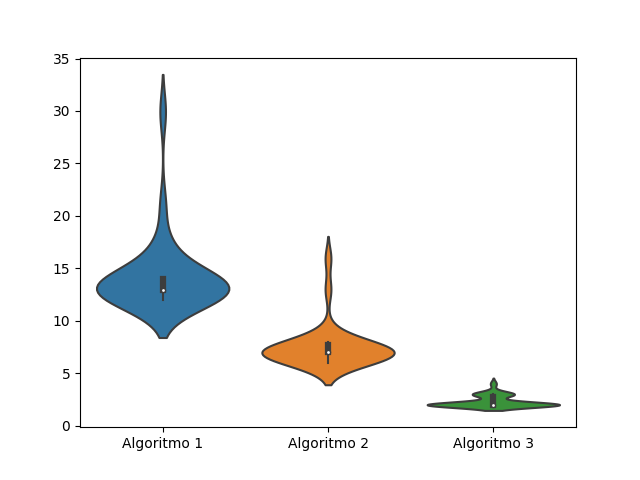
\includegraphics[width=\textwidth]{AlgorithmVariation.png}
         \caption{Variaci\'on del algoritmo}
         \label{fig:varalg}
     \end{subfigure}
     \begin{subfigure}[b]{0.49\textwidth}
         \centering
         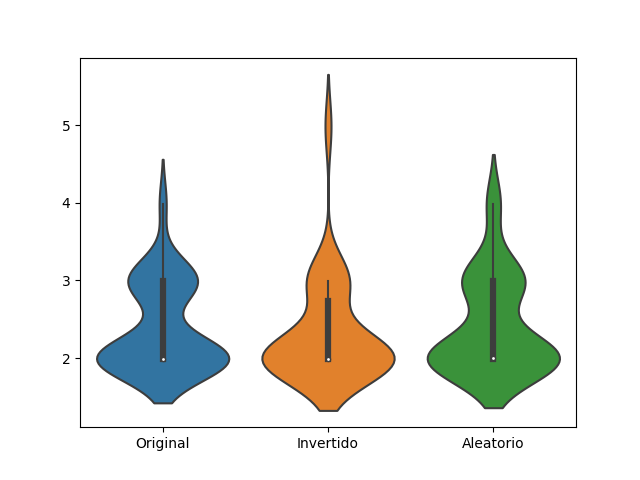
\includegraphics[width=\textwidth]{OrderVariation.png}
         \caption{Variaci\'on del orden}
         \label{fig:varord}
     \end{subfigure}
     \caption{Diagramas viol\'in}
     \label{diag}
\end{figure}

\newpage

\section{Conclusiones}\label{con}
Tomando en cuenta un valor de $p<0.05$ como prueba de que la diferencia en tiempos de ejecuci\'on es significativa, entonces se tiene que: 1) Hay una clara dependencia entre el algoritmo utilizado y el tiempo que toma encontrar los n\'umero primos, y 2) la media de los tiempos de ejecuci\'on al variar el orden inicial no parece presentar una diferencia significativa.

Esto puede ser m\'as evidente al observar los diagramas presentados. En la figura \ref{fig:varalg} se observa claramente la disminuci\'on de las medias (representadas por el punto blanco), al utilizar un algoritmo m\'as eficiente. Por otro lado, en la figura \ref{fig:varord} las medias se encuentran en posiciones muy similares, adem\'as de que las distribuciones para cada orden no son tan distintas.
\bibliography{tarea_3}
\bibliographystyle{plainnat}
\end{document}
